\documentclass{beamer}

\usepackage{beamerthemesplit}
\usetheme{Warsaw}

\title{PGQ, Pretty Darn Quick}
\author{Dimitri Fontaine, Title by Selena Deckelmann}
\date{May 22, 2009}

\begin{document}

\frame{\titlepage}

\section*{Outline}
\frame{
  \frametitle{Table of contents}
  \tableofcontents
}

\section{Batches needs}

\begin{frame}[fragile]
  \frametitle{Database processing oriented batches}

\begin{columns}[c]

\column{.5\textwidth}

If you're managing an \textit{OLTP} system, you probably have out of line
processing to get done, and probably are using cron batches and home made
\textit{daemons}.

\pause
\begin{example}
\begin{verbatim}
  while( true ) {
    // what a nice daemon!
  }
\end{verbatim}
\end{example}

\pause
\column{.5\textwidth} 
  Of course you want them 
  \begin{itemize}
   \item<3-> reliable, easy to monitor and control (logs)
   \item<4-> out of a developer \texttt{screen} session
   \item<5-> easy to stop \& restart
   \item<6-> to reuse existing models
  \end{itemize}

\end{columns}
\end{frame}

\section{PGQ features}

\frame{
  \frametitle{Reusing Open-Source code?}

  PGQ is a \alert{queuing} solution implemented as a PostgreSQL extension
  module, providing an \texttt{SQL} and a \texttt{python} API. It offers the
  producer multi consumers subscribtion model and is the transport layer of
  the \texttt{londiste} replication solution.

  \pause
  PGQ is
  \begin{itemize}
   \item<2-> performant (maintaining 3 tables, using \texttt{TRUNCATE})
   \item<3-> easy to install and monitor
   \item<4-> robust
  \end{itemize}
}

\section{Mix and Match}

\frame{
  \frametitle{Implementing a daemon atop PGQ}

  Skytools comes with two \textit{middleware} for you to abuse to make
  daemons with, the \texttt{python} \textit{DBScript} facility and the
  \texttt{PHP} \textit{libphp-pgq} one. \linebreak

  \pause
  For the \texttt{python} version see resources on the internet. Here we're
  dealing with the \texttt{PHP} one. \texttt{PHP} is inferior a language but
  we sometime have to support it, to leverage existing model classes.

}

\begin{frame}[fragile]
  \frametitle{libphp-pgq}

  You subclass a \texttt{PGQConsumer} superclass and implement two methods:
  \begin{itemize}
   \item \texttt{config}
   \item \texttt{process\_event}
  \end{itemize}

  \pause

  The transaction \texttt{BEGIN} and \texttt{COMMIT} are managed by the
  class you inherited code from, just process data and return one of

  \begin{verbatim}
    PGQ_EVENT_OK
    PGQ_EVENT_FAILED
    PGQ_EVENT_RETRY
    PGQ_ABORT_BATCH
  \end{verbatim}
\end{frame}

\begin{frame}[fragile]
  \frametitle{libphp-pgq abstract classes}

  Different main classes are available for you to subclass, depending on
  what you want to do. Some documentation is available online at
  http://pgsql.tapoueh.org/pgq/pgq-php/

  \begin{itemize}
   \item<2-> \texttt{PGQConsumer}
   \item<3-> \texttt{PGQRemoteConsumer}
   \item<4-> \texttt{PGQEventRemoteConsumer}
  \end{itemize}
  

\end{frame}

\section{Conclusion}

\begin{frame}[fragile]
  \frametitle{Gone live!}

  We have several \texttt{PGQ} daemons in our live environments, monitored
  with \texttt{nagios} and \texttt{munin}, and we're able to easily control
  them. It's much better than previously.

  \pause

\begin{columns}[c]
\column{.5\textwidth}
  \begin{example}
  \begin{verbatim}
    # mydaemon.php start
    # mydaemon.php status
    # mydaemon.php logmore

    # mydaemon.php kill
  \end{verbatim}
  \end{example}
\column{.5\textwidth} 
\begin{center} 
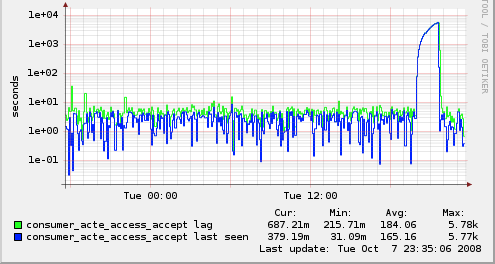
\includegraphics[height=1.3in]{pgq.png}
\end{center} 
\end{columns}
\end{frame}

\end{document}
